\documentclass{cmspaper}
\usepackage{graphicx}
\usepackage{rotate}
\usepackage{relsize}
\usepackage{lineno}

\newcommand{\met} {\ensuremath{E\!\!\!\!/_T}}
\newcommand{\ttbar} {\ensuremath{t\bar{t}~}}
\newcommand{\ptll} {\ensuremath{P_T(\ell\ell)}}
\newcommand{\ptllres} {\ensuremath{P^{\rm res}_T(\ell\ell)}}
\def\ack{\section*{Acknowledgments}}

\linenumbers

\begin{document}

%==============================================================================
% title page for many authors
%
\begin{titlepage}
\title{Search for Supersymmetry in same sign dilepton final states with b Jets and Missing Energy at the LHC}

  \begin{Authlist}
    D.~ Barge, C.~Campagnari, P.~Kalavase, D.~Kovalskyi, V.~Krutelyov, J.~Ribnik
    \Instfoot{ucsb}{University of California, Santa Barbara}
    W.~Andrews, G.~Cerati, D.~Evans, F.~Golf, I.~MacNeill, S.~Padhi, Y.~Tu, F.~W\"urthwein, A.~Yagil, J.~Yoo
    \Instfoot{ucsd}{University of California, San Diego}
    L.~Bauerdick, I.~Bloch, K.~Burkett, I.~Fisk, Y.~Gao, O.~Gutsche, B.~Hooberman, S.~Jindariani, J.~Linacre
    \Instfoot{fnal}{Fermi National Accelerator Laboratory, Batavia, Illinois}
  \end{Authlist}

\begin{abstract}
We search for supersymmetry in same sign dilepton final states with at least two b jets 
and large \met~. The search is performed in a data sample collected with the CMS detector
of pp collisions at a centre-of-mass energy of 7 TeV, corresponding to an integrated
luminosity of $349$ pb$^{-1}$. For these searches, the dominant background is from \ttbar 
events. No excess above the standard model background expectation is observed.
Upper limits at 95\% confidence level are set on the number of observed events.
%pMSSM as well as the simplified models 
%involving stop and sbottom productions.
\end{abstract}
\end{titlepage}

\section{Introduction}
\label{sec:intro}

After the successful operation of the Large Hadron Collider (LHC) and the CMS detector
in 2010 and 2011, and with good prospects for the future, the LHC is now ready to shed light on a number 
of open questions in Particle Physics 
such as the mechanism of electroweak (EW) symmetry breaking, or the 
new physics, Beyond the Standard Model (BSM), that stabilizes the EW scale. 

A wealth of theories that extend the Standard Model have been put forth during the past decades. Supersymmetry (SUSY) is
arguably the best motivated BSM theory --- and certainly the most 
thoroughly studied. 
Indeed, searches for SUSY are among the primary objectives of the 
CMS experiment. SUSY is exceedingly popular not 
only for its theoretical beauty but also because SUSY phenomenology 
is extremely rich, 
%in fact is can mimic almost any other new physics scenario. 
leading to a large variety of possible new signals at the LHC. 
In spite of this, the majority of SUSY studies focus on a very special 
setup: the so-called Constrained Minimal Supersymmetric Standard Model (CMSSM). 
This was justified in the preparation for discoveries as the CMSSM, 
having just a handful of new parameters, is very predicive. However, 
the simplifying assumption of universality at the GUT scale lacks a sound 
theoretical motivation. Consequently, the CMSSM should be regarded as a showcase 
model. When it comes to interpreting experimental results, it is reasonable and interesting to do this within the CMSSM because it 
provides (to some degree) an easy way to show performances, 
compare limits or reaches, etc. However, the interpretation of experimental results in the 
$(m_0,m_{1/2})$ plane risks imposing unwarranted constraints on SUSY, as many 
mass patterns and signatures that are possible a priori are not covered in the CMSSM. 
The same problem arises in any analysis that assumes a particular 
SUSY breaking scheme. 

In this document, we therefore introduce a different approach, which uses only 
minimal assumptions on the underlying SUSY parameters. In particular, given the absence of experimental guidance, we choose
not to rely on a particular SUSY breaking scheme.
Instead, we use a 19-dimensional 
parametrization of the MSSM, called the \emph{phenomenological MSSM} (pMSSM),
with parameters defined not at the GUT scale but instead at the SUSY scale 
(by convention the geometric mean of the two stop masses).
We demonstrate the feasibility of our approach by applying it to 
the 2011 CMS data-set corresponding to 1~fb$^{-1}$ of integrated luminosity.  
Using profile likelihoods, we combine 
the dijet $\alpha_T$ analysis, the opposite-sign dilepton 
analysis and the same-sign dilepton analysis and derive constraints 
on the SUSY particles with as few simplifying assumptions as possible.
Results from other SUSY analyses in CMS will be added as soon as they become available.

We first give the motivation to go beyond the CMSSM and work in 
a generic MSSM setup. After this, the pMSSM and its parametrization is defined. 
We then outline our analysis, giving details on the pMSSM points we have used, 
the detector simulation and the CMS analyses, and describe the statistical method based on 
profile likelihoods used for coping with the 19-dimensional model. Finally, we discuss our results and summarize our conclusions.


%\section{Simulated Event samples}
\label{sec:mcsignal}

In the MSSM, the scalar partners of the left- and right-handed squarks, $\tilde{q_L}$
and $\tilde{q_R}$, can mix to form mass eigenstates. These mixing effects thus leads to different fermion
masses and therefore becomes important for the third generation. The large mixing can yield sbottom ($\tilde{b_1}$)
and stop ($\tilde{t_1}$) eigenstates which are significantly lighter than other squarks. This also implies  $\tilde{b_1}$
and $\tilde{t_1}$ could be produced with larger cross sections then the light flavour squarks at the LHC. Consequently, 
the subsequent decays of $\tilde{b_1}$ and $\tilde{t_1}$ can lead to same sign dileptons in association with b quarks.
Furthermore, the $\tilde{g}\tilde{g}$ productions via $\tilde{\chi}^\pm_1$ such as $\tilde{g} \rightarrow \tilde{\chi}^{+}_{1} b \bar{t}$
can also give rise to same sign dileptons with b jets.

\section{Search for same-sign dileptons with $b$ jets}
\label{searchbtag}

This analysis is based on the inclusive same-sign dilepton search documented in AN-2011/258~\cite{ssnote2011} and corresponds to an
integrated luminosity of 349 pb$^{-1}$. In that study we searched for events with two isolated same-sign leptons
in association with 2 additional jets and \met. Here we re-use most of the baseline event selection~\footnote{The additional 
$Z$ veto is not applied in this study}. In addition, we require at least 2 b-tagged jets using Track Counting High Efficiency 
Medium (TCHEM) working point tagger~\cite{BTVPAS2011}. We refer to TCHEM with the requirement that three of the tracks have $IP$ 
significance $ > 3.3$. For this tagger the b-tagging efficiency is $0.62 \pm 0.01$ and the acceptance of light flavor jets 
is $0.018 \pm 0.004$~\cite{BTVPAS2011}.

\subsection{Event Selection}
\label{eventsel}

The event selection for high p$_T$  and low p$_T$ baseline regions are briefly summerized as follows:

\begin{itemize}
\item At least two isolated same-sign leptons ($ee$, $e\mu$, and $\mu\mu$) with $|\eta| < 2.4$
\begin{itemize}
\item For the high-$p_T$ study, both leptons are required to be $p_T > 10$ GeV, with one of them $p_T > 20$ GeV.
\item For the low-$p_T$ study, the electrons are required to be $p_T > 10$ GeV and muons $p_T > 5$ GeV.
\end{itemize}
\item At least two particle flow jets tagged using TCHEM tagger with $p_T > 40$ GeV and $|\eta| < 2.4$ corrected with L1FastL2L3 corrections.
\item The selected jets must be separated from the lepton by $\Delta R > 0.4$.
\item The scalar sum of momenta $H_T > 80$ ($H_T > 200$) GeV is required for high-$p_T$ (low-$p_T$) analysis.
\item \met $> 30$ GeV.
\item We remove dilepton events with invariant mass $M_{ll} < 5$ GeV.
\end{itemize}

More details are found in Reference~\cite{ssnote2011}.

\subsection{Event Yields and Background Estimation}
\label{eventsel}

The results of this search in the above-mentioned kinematical region are summerized in Table~\ref{tab:ssyields1},~\ref{tab:ssyields2}. Data-driven background 
predictions are used to estimate SM backgrounds. This is based on a combination of estimating ``Tight-To-Loose ratio'' (Fake Rate)
and electron charge mis-reconstruction rate (Charge Flip rate). The probability for muons to be reconstructed 
with the wrong sign in the relevant momemtum range is negligible.

The event yields have the following characteristics:

\begin{itemize}
\item The contributions from rare processes such as $qqW^\pm W^\pm, WWW, t\bar{t}W$, and double parton $W^\pm W^\pm$ are negligibly small.
\item The diboson backgrounds $WW, WZ$, and $ZZ$ are found to be negligible.
\item The prediction from fake rates includes the systematic error of 50\%.
\item The prediction from flip rates incldues the systematic error of 25\%.
\item The systematic errors are added when propagting the fake/flip rates into the total prediction.
\item We do not consider any MC driven estimation for the final prediction.
\end{itemize}

\vspace{6 mm}
\begin{table}[htb]
\begin{center}
\begin{tabular}{|c|c|c|c|c|}
\hline
Sample & $e^{\pm}e^{\pm}$    & $\mu^{\pm}\mu^{\pm}$ & $e^{\pm}\mu^{\pm}$      & total \\ \hline
% all the MCs
\hline
\ttbar\  & 0.15 $\pm$ 0.09 & 0.25 $\pm$ 0.11 & 0.25 $\pm$ 0.11 & 0.65 $\pm$ 0.18 \\ 
Single top  & 0.02 $\pm$ 0.02 & 0.02 $\pm$ 0.02 & 0.02 $\pm$ 0.01 & 0.06 $\pm$ 0.03 \\ 
wjets  & 0.00 $\pm$ 0.00 & 0.00 $\pm$ 0.00 & 0.00 $\pm$ 0.00 & 0.00 $\pm$ 0.00 \\ 
DY  & 0.00 $\pm$ 0.00 & 0.00 $\pm$ 0.00 & 0.00 $\pm$ 0.00 & 0.00 $\pm$ 0.00 \\ 
VV  & 0.00 $\pm$ 0.00 & 0.00 $\pm$ 0.00 & 0.00 $\pm$ 0.00 & 0.00 $\pm$ 0.00 \\ 
\hline
Total MC  & 0.17 $\pm$ 0.09 & 0.27 $\pm$ 0.11 & 0.27 $\pm$ 0.11 & 0.71 $\pm$ 0.18 \\
\hline\hline
data  (349 pb$^{-1}$)     & 1  &  1  & 0  & 2      \\ \hline
fake rate prediction & & & & \\ \hline
single fake   & 0.38 $\pm$ 0.38 & 0.52 $\pm$ 0.37 & 0.00 $\pm$ 0.00 & 0.90 $\pm$ 0.52 (3 evts) \\
double fake   & 0.00 $\pm$ 0.00 & 0.00 $\pm$ 0.00 & 0.00 $\pm$ 0.00 & 0.00 $\pm$ 0.31 (0 evts) \\
fake prediction & 0.38 $\pm$ 0.38 & 0.52 $\pm$ 0.37 & 0.00 $\pm$ 0.00 & 0.90 $\pm$ 0.60 \\
\hline\hline
flip rate prediction & $0.05 \pm 0.01$ & 0 & $0.06\pm 0.02$ & $0.11\pm 0.03$ \\ \hline
total fake rate prediction & $0.38 \pm 0.43$ & $0.52\pm 0.45$ & $0.00 \pm 0.00$ & $0.90 \pm 0.69$ \\ \hline
total bkg prediction & $0.43\pm 0.43$ & $0.52 \pm 0.45$ & $0.06 \pm 0.2$ & $1.01\pm 0.75$ \\\hline
\end{tabular}
\caption{\protect Data and Monte Carlo yields for the same-sign high-$p_T$ dileptons with $H_T > 80$ GeV and \met $> 30$ GeV. Uncertainties in 
the lower three rows also include the systematic uncertanities on the method used.\label{tab:ssyields1} }
\end{center}
\end{table}

\vspace{6 mm}
\begin{table}[htb]
\begin{center}
\begin{tabular}{|c|c|c|c|c|}
\hline
Sample & $e^{\pm}e^{\pm}$    & $\mu^{\pm}\mu^{\pm}$ & $e^{\pm}\mu^{\pm}$      & total \\ \hline
% all the MCs
\hline
\ttbar\  & 0.15 $\pm$ 0.09 & 0.25 $\pm$ 0.11 & 0.30 $\pm$ 0.19 & 0.70 $\pm$ 0.19 \\ 
Single top  & 0.02 $\pm$ 0.02 & 0.02 $\pm$ 0.02 & 0.02 $\pm$ 0.01 & 0.06 $\pm$ 0.03 \\ 
wjets  & 0.00 $\pm$ 0.00 & 0.00 $\pm$ 0.00 & 0.00 $\pm$ 0.00 & 0.00 $\pm$ 0.00 \\ 
DY  & 0.00 $\pm$ 0.00 & 0.00 $\pm$ 0.00 & 0.00 $\pm$ 0.00 & 0.00 $\pm$ 0.00 \\ 
VV  & 0.00 $\pm$ 0.00 & 0.00 $\pm$ 0.00 & 0.00 $\pm$ 0.00 & 0.00 $\pm$ 0.00 \\ 
\hline
Total MC  & 0.17 $\pm$ 0.09 & 0.27 $\pm$ 0.11 & 0.32 $\pm$ 0.19 & 0.76 $\pm$ 0.19 \\
\hline\hline
data  (349 pb$^{-1}$)     & 0  &  1  & 0  & 1      \\ \hline
fake rate prediction & & & & \\ \hline
single fake   & 0.00 $\pm$ 0.00 & 0.00 $\pm$ 0.00 & 0.00 $\pm$ 0.00 & 0.00 $\pm$ 0.56 (0 evts) \\
double fake   & 0.00 $\pm$ 0.00 & 0.51 $\pm$ 0.30 & 0.00 $\pm$ 0.00 & 0.51 $\pm$ 0.30 (3 evts) \\
fake prediction & 0.00 $\pm$ 0.00 & 0.51 $\pm$ 0.30 & 0.00 $\pm$ 0.00 & 0.51 $\pm$ 0.63 \\
\hline\hline
flip rate prediction & $0.01 \pm 0.004$ & 0 & $0.02\pm 0.006$ & $0.03\pm 0.01$ \\ \hline
total fake rate prediction & $0.00 \pm 0.00$ & $0.51\pm 0.68$ & $0.00 \pm 0.00$ & $0.51 \pm 0.68$ \\ \hline
total bkg prediction & $0.01\pm 0.004$ & $0.51 \pm 0.68$ & $0.02 \pm 0.006$ & $0.54 \pm 0.68$ \\\hline
\end{tabular}
\caption{\protect Data and Monte Carlo yields for the same-sign low-$p_T$ dileptons with $H_T > 200$ GeV and \met $> 30$ GeV. Uncertainties in 
the lower three rows also include the systematic uncertanities on the method used.\label{tab:ssyields2} }
\end{center}
\end{table}

The dominant SM contribution in both low- and high-$p_T$ selections are found to be from \ttbar\ decays. The estimation
is in a good agreement with the observation. We also note that the backgrounds with respect to the inclusive same sign
dilepton search is suppressed by an order of magnitude due to the b-tag requirements.

\subsection{Discussion of Backgrounds}
\label{bkgdiscussion}

As shown earlier, the primary source of background events are from \ttbar\ decays, which are estimated using the fake rate method. Here we further investigate 
by performing a closure test on a large \ttbar\ sample~\footnote{The POWHEG sample TTToLNu2Q2B\_7TeV-powheg-pythia6\_Spring11-PU\_S1\_START311\_V1G1-v1 is only used for the 
closure test. In this sample the $W \rightarrow l \nu$ is already forced at the generator level.} corresponding to a luminosity normalization of 1fb$^{-1}$. The fake 
rates for electrons and muons are determined from the QCD sample~\cite{ssnote2011}. This test is meant to check if the fake rate, as determined from the QCD events 
can be applied to \ttbar\ with at least 2 b-tagged jets. 

We classify them as follows, based on truth matched to their ``parents'':
\begin{itemize}
\item Type-I: both leptons originate from real $W$ (including $W \rightarrow \tau \rightarrow l$) bosons, one with 
mis-reconstructed charge.
\item Type-II a): one of the leptons is from a real $W$ and the other originates from heavy flavor sources ($b,c$).
\item Type-II b): one of the leptons is from a W and the other is a fake lepton from light flavor sources.
\item Type-III: both leptons are fakes.
\end{itemize} 

\begin{table}[hbt]
\begin{center}
\begin{tabular}{|l|c|c|c|c|c|c|}\hline
Same Sign Leptons & Total &      Type-I &  Type-II & Type-II a) & Type-II b) & Type-III \\ \hline

$ee$ & 0.31$\pm$0.07 & 0.00$\pm$0.00 & 0.31$\pm$0.07 & 0.11$\pm$0.04 & 0.21$\pm$0.05 & 0.00$\pm$0.00 \\
$\mu\mu$ & 0.26$\pm$0.06 & 0.00$\pm$0.00 & 0.26$\pm$0.06 & 0.22$\pm$0.05 & 0.04$\pm$0.04 & 0.00$\pm$0.00 \\
$e\mu$ & 0.57$\pm$0.09 & 0.00$\pm$0.00 & 0.57$\pm$0.09 & 0.37$\pm$0.07 & 0.21$\pm$0.05 & 0.00$\pm$0.00 \\
total & 1.15$\pm$0.13 & 0.00$\pm$0.00 & 1.15$\pm$0.13 & 0.70$\pm$0.10 & 0.45$\pm$0.08 & 0.00$\pm$0.00 \\ \hline

\end{tabular}
\caption{ Expected number of \ttbar\ events, of various types in 1 fb$^{-1}$ of integrated luminosity. Uncertainties are from MC statistics.\label{tab:fakeOrigin1}}
\end{center}
\end{table}

\begin{table}[hbt]
\begin{center}
\begin{tabular}{|l|c|c|c|c|c|c|}\hline
Same Sign Leptons & Total &      Type-I &  Type-II & Type-II a) & Type-II b) & Type-III \\ \hline

$ee$ & 0.39$\pm$0.03 & 0.00$\pm$0.00 & 0.39$\pm$0.03 & 0.20$\pm$0.02 & 0.19$\pm$0.03 & 0.00$\pm$0.00 \\
$\mu\mu$ & 0.36$\pm$0.03 & 0.00$\pm$0.00 & 0.36$\pm$0.03 & 0.30$\pm$0.03 & 0.06$\pm$0.01 & 0.00$\pm$0.00 \\
$e\mu$ & 0.76$\pm$0.05 & 0.00$\pm$0.00 & 0.76$\pm$0.05 & 0.54$\pm$0.04 & 0.22$\pm$0.03 & 0.00$\pm$0.00 \\
total & 1.51$\pm$0.06 & 0.00$\pm$0.00 & 1.51$\pm$0.06 & 1.04$\pm$0.05 & 0.47$\pm$0.04 & 0.00$\pm$0.00 \\ \hline

\end{tabular}
\caption{ Predicted number of \ttbar\ events, of various types in 1 fb$^{-1}$ of integrated luminosity. Uncertainties are from MC statistics.\label{tab:fakeOrigin2}}
\end{center}
\end{table}

Tables~\ref{tab:fakeOrigin1} and~\ref{tab:fakeOrigin2} show the estimated and predicted event yields. We predict within 50\% the Type-II contributions, where one of
the leptons is from a real $W$ and the other is a fake lepton. Within the Type-II the largest source of uncertanity is due to overprediction of Type-II a) 
component of the background, where we expected one of the leptons to be originated from heavy flavor sources $(b, c)$.

Another possible source of \ttbar\ background could be due to the residual jet from the semi-leptonic $b \rightarrow c$ decays. We expect this
residual b-jet to be vetoed using the overlap removal between the lepton and the jet. In order to study this effect, we relax the $\Delta R$
requirement between the lepton and the b-tag jet. 

\begin{figure}[htb]
\begin{center}
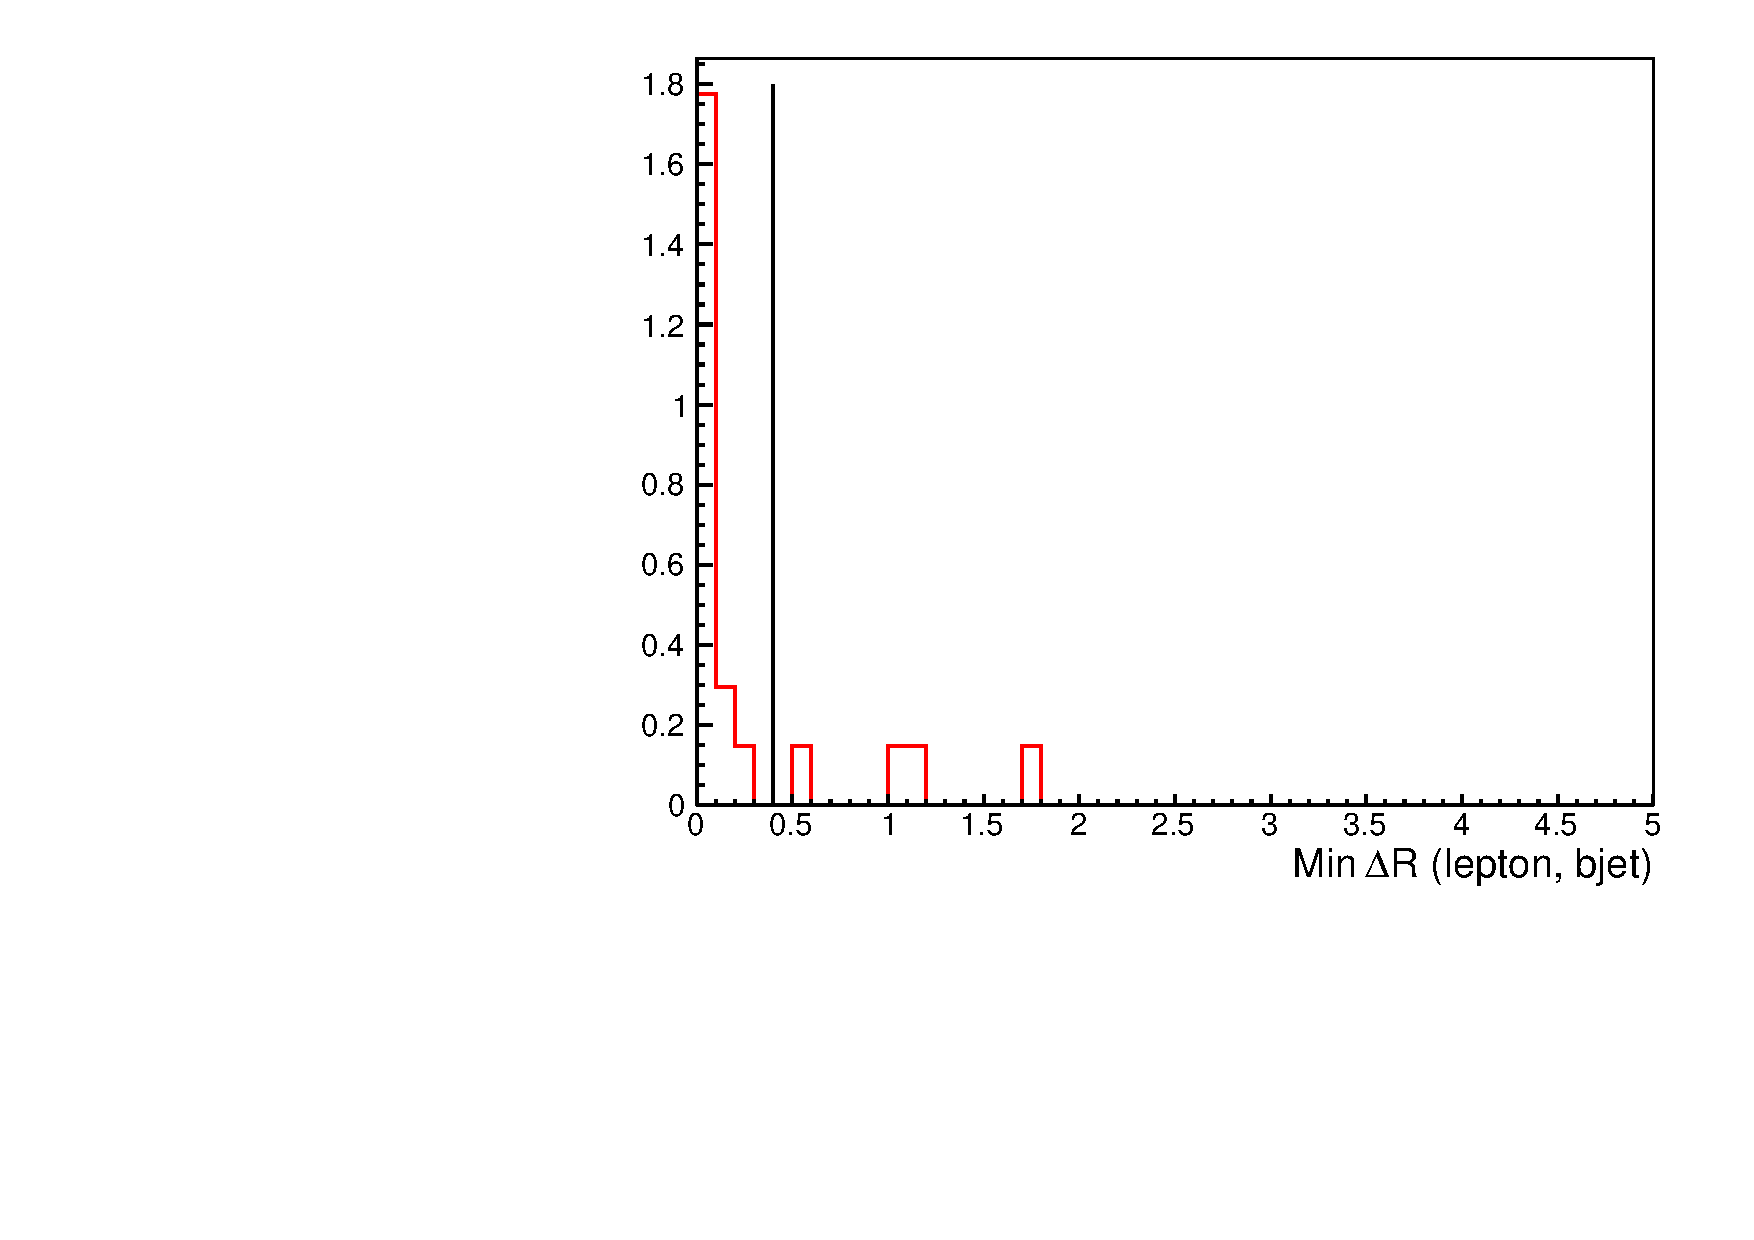
\includegraphics[width=0.6\linewidth, height=0.4\linewidth]{figs/bjetlepton.pdf}
\caption{ Minimum $\Delta R$ between the lepton and the b-tag jet in \ttbar\ decays.\label{fig:ttbar_residual}}
\end{center}
\end{figure}

Fig.~\ref{fig:ttbar_residual} shows that the bulk of such events in \ttbar\ decays are well within the $\Delta R < 0.4$ between lepton and the b-jet.



 





\section{Acceptance Systematics}
\label{sec:systematic}
Systematic uncertainties arise from uncertainties on event selections expected in simulation 
compared to the actual performance of  the detector. 
As this search is in many ways similar to the inclusive same-sign dilepton search~\cite{ssnote2011}, 
our treatment of efficiency systematics parallels the one in that analysis.
In this section, we briefly summarize those results, and
describe the uncertanities due to the b-tagging requirement.

The only new source of systematics in this analysis is from the uncertainty on the
b-jet tagging efficiency.
As already mentioned in Section~\ref{sec:bjetSF}, this uncertainty
is 4 (14)\% for jets with $\pt<240 (>240)~\GeV$.
As an illustration of the b-jet momentum distribution,
we compare them in Fig.~\ref{fig:lm9ttbar} for  \ttbar\ events (before the same-sign requirement)
and for the LM9 cMSSM SUSY benchmark point.\footnote{
The LM9 point is defined by the common scalar mass (m0) $ = 1.45$ TeV, 
the common gaugino mass (m1/2) = 175 GeV, the ratio of the Higgs expectation
values (tan$\beta)  = 10$, tri-linear coupling (A0) = 0 and the  sign of the Higgsino mass parameter ($\mu) > 0$. 
}
While most of the b-jets from \ttbar\ are below 240~\GeV, those from LM9
have a large contribution from higher momenta.
Our target searches include final states with two or more b-quark jets.
This means the efficiency to select two b-jets, as well as its uncertainty
varies among the signal final states considered
\begin{itemize}
\item same-sign top pair production, as from $Z^\prime$ exchange,
	is similar in topology to that of the opposite-sign \ttbar\ production
	and has only two b-jets in the final state with most of them with $\pt<240~\GeV$.
	The b-tagging efficiency is then approximately 10\%
	and the corresponding per-event scale factor is $0.922 \pm 0.092$.
\item direct sbottom pair production has two b-jets in the final state
	with a large fraction of b-jets with $\pt>240~\GeV$.
	The b-tagging efficiency scale factor is still 0.922, but its uncertainty
	varies among the signal model points from as low as 10\%
	to as high as 30\%.
	This uncertainty is evaluated event-by-event and then point-by-point in the limit setting procedure.
\item gluino pair production with stops in the final states considered
	here all have four b-jets in the final state.
	Now the efficiency scale factor changes as well
	depending on the number of b-jets in the acceptance.
	This is evaluated event-by-event and point-by point in the limit setting procedure.
\end{itemize}


\begin{figure}[htb]
\begin{center}
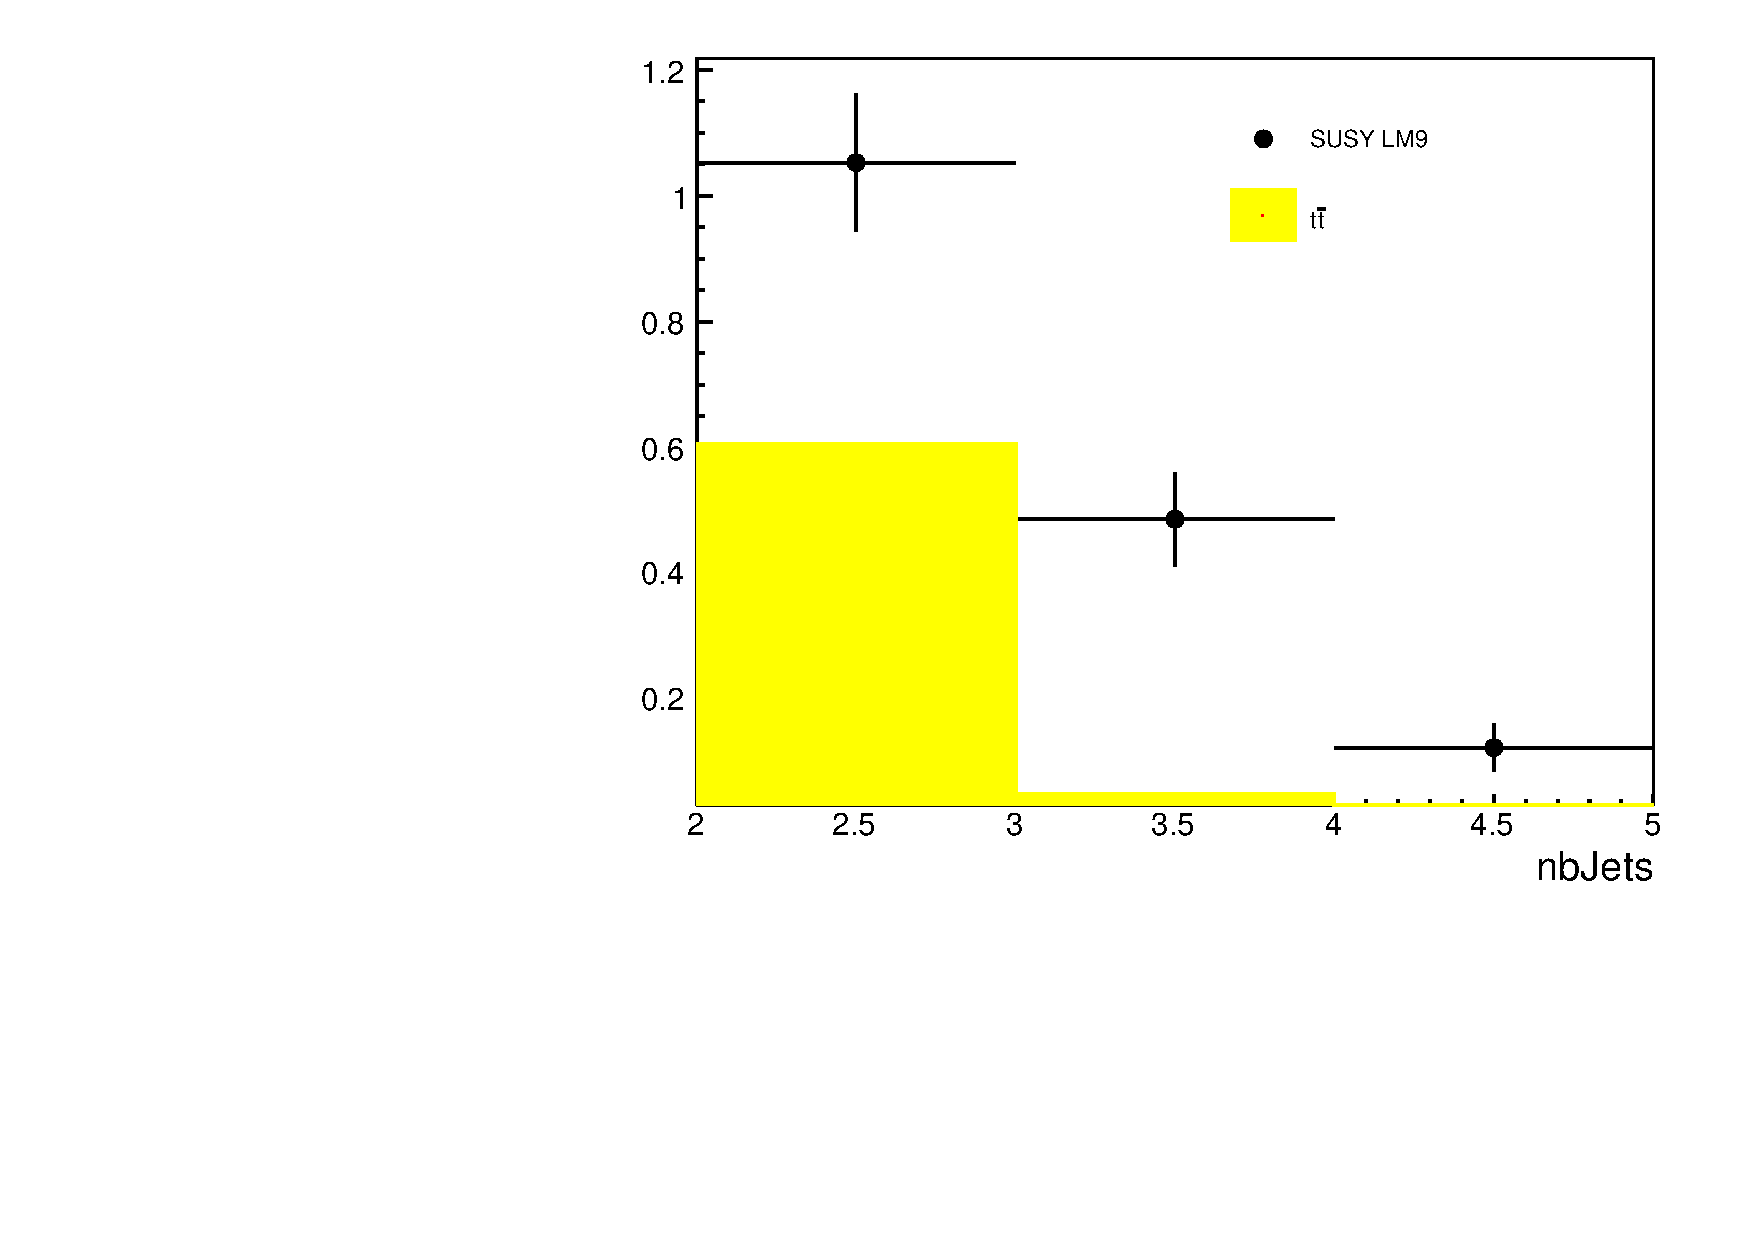
\includegraphics[width=0.48\textwidth]{figs/lm9.pdf}
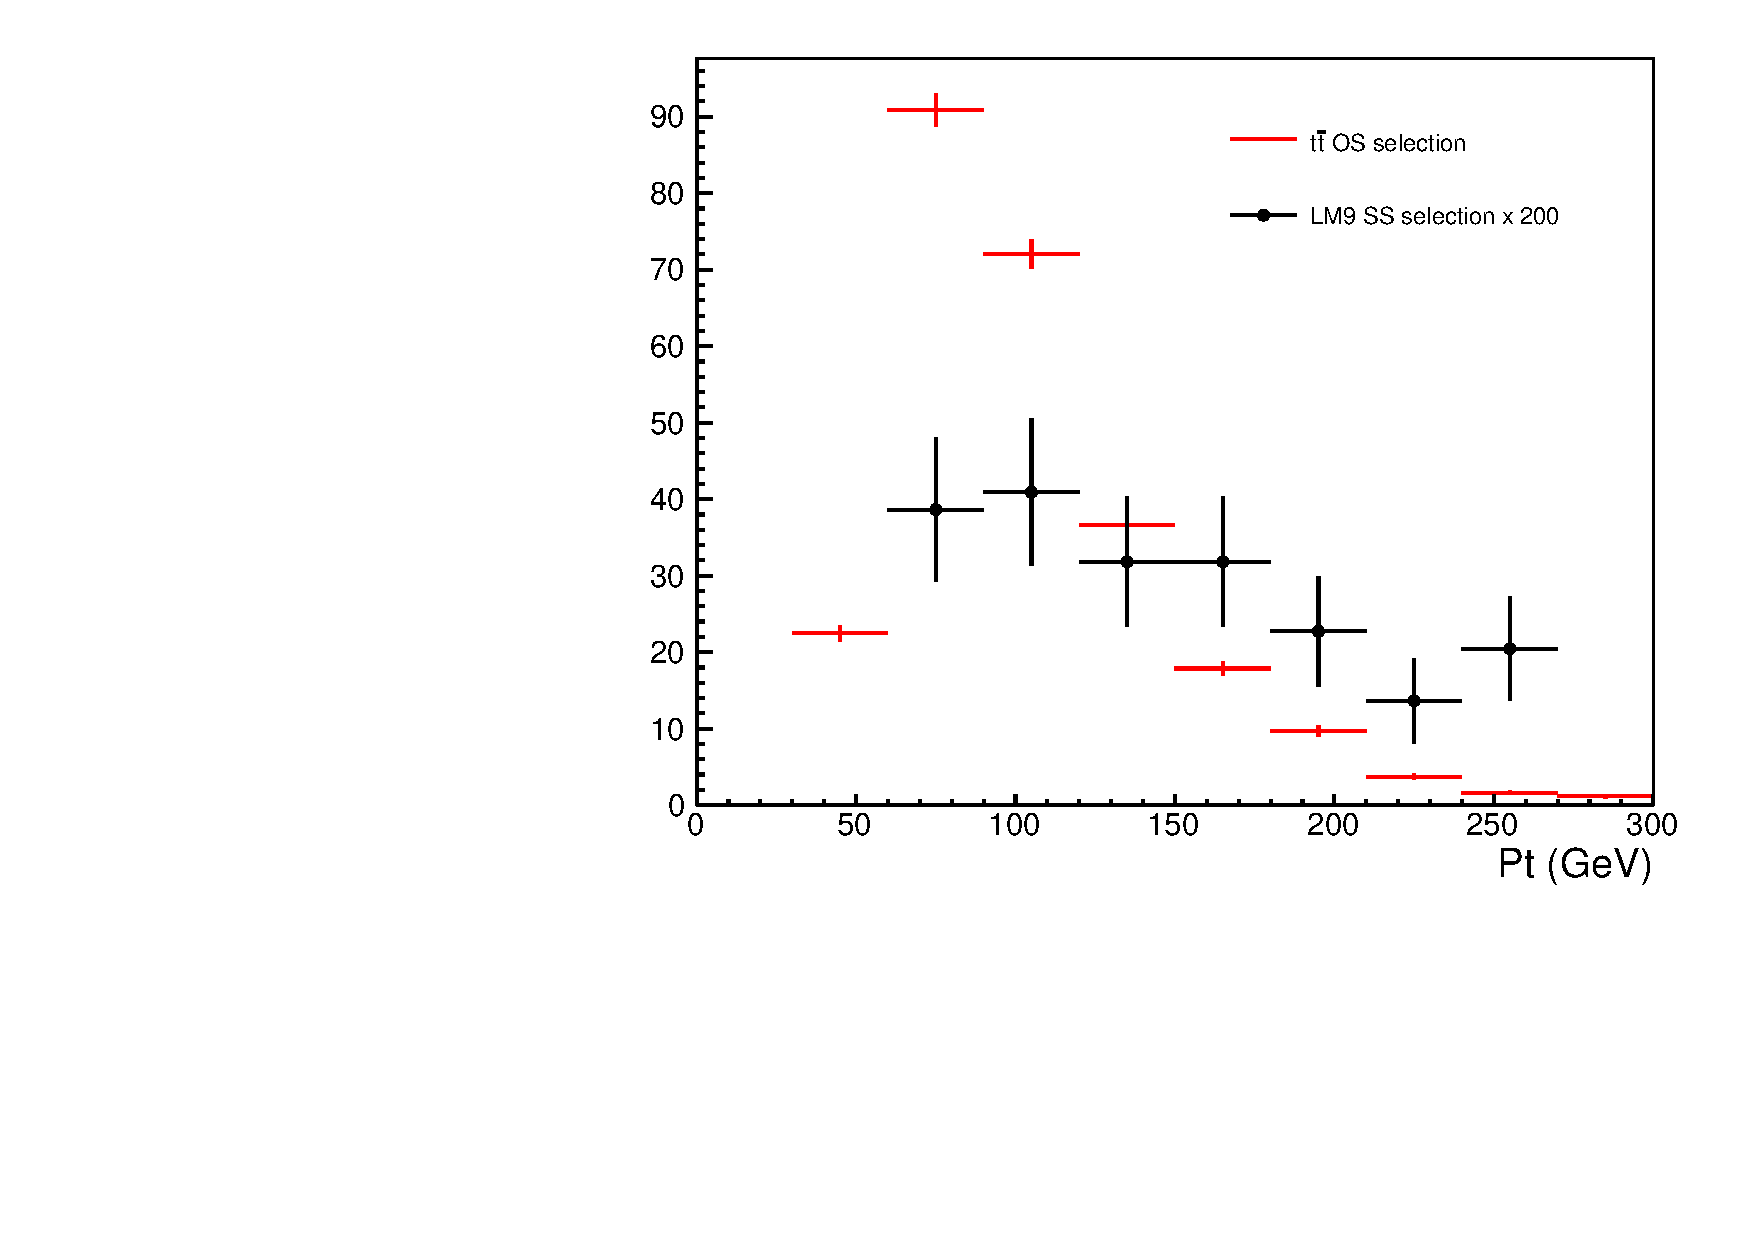
\includegraphics[width=0.48\textwidth]{figs/bjetleading.pdf}
\caption{ Differential distributions of leading b-tag jet $\pt$ for the 
LM9 benchmark point and \ttbar\ simulations.
The normalization is arbitraty.\label{fig:lm9ttbar}}
\end{center}
\end{figure}


A summary of systematic uncertainties is given in Table~\ref{tab:systSumm}.
Here the b-tagging systematics is applicable only to the same-sign top production signature.

\begin{table}[h]
\begin{center}
\caption{\small\label{tab:systSumm}Summary of systematic uncertainties on the signal selection and
expectation. 
Reported values are fractional, relative to the total cross section.
The energy scale, b-tagging, and PDF uncertainties are calculated separately in every model point.
These uncertainties quoted here are relevant to the $Z^\prime$ model.}
\begin{tabular}{lcccc}\hline
Source 					& $ee$		& $\mu\mu$		& $e\mu$	& all 	\\ \hline
Lepton selection			& 12\%		& 12\%			& 11\%		& 11\% 	\\
Energy scale				& 8\%		& 8\%			& 8\%		& 8\% 	\\
ISR/FSR and PDF				& 2\%		& 2\%			& 2\%		& 2\% 	\\
b-tag selection                         & 8\%          	& 8\%                   & 8\%           & 8\% 	\\
Total without luminosity		& 17\%		& 17\%			& 17\%		& 17\%	\\ \hline
Integrated luminosity			& 4.5\%		& 4.5\%			& 4.5\%		& 4.5\%	\\ \hline
Total 					& 17\%	 	& 17\%	 		& 17\% 		& 17\% 	\\
\hline
\end{tabular}
\end{center}
\end{table}

\subsection{Event-by-Event B-tagging scale factor and associated systematic uncertainty}
We evaluate an event-by-event btagging scale factor ($SF_{\rm event}$) as follows:

\begin{itemize}
\item for each MC event passing the event selection we start
from the scale factors $SF_i$ associated with the two or more
tagged jets.  Note that $SF_i$ can in principle be a function 
of jet $\eta$, $\pt$, etc.  Following the btag group recommendations,
for now it is taken as a constant: $SF=0.96$.

\item For events with two btagged jets: $SF_{\rm event}=SF^2$.

\item For events with three btagged jets: $SF_{\rm event}=SF^3 + 3SF^2(1-SF)$.

\item For events with four btagged jets: $SF_{\rm event}=SF^4 + 4SF^3(1-SF) + 6SF^2(1-SF)^2$.
\end{itemize}

Note that the procedure above would not work if $SF>1$, but this is not an issue
since $SF=0.96$.
It also implicitely assumes that all btags are from b-quarks.  For the models under 
consideration, we have verified that the MC contribution to the acceptance from 
events that need at least one tag from $udsgc$ in order to pass the $\ge$ 2 tags 
requirements is small.  For example, in the $Z'$ model, this contribution is
only $\approx$ 4\%.  Note that the bias in $SF_{\rm event}$ due to the improper traeatment
these events is 4\% times some quantity proportional to the difference in scale 
factors between $b$-jets and $usdgc$ jets.  Therefore, it is $<<$ 4\% and we think
can be ignored.  

In order to calculate the uncertainty ($\delta SF$) on the event-by-event $SF_{\rm total}$,
we also need the single jet btagging efficiency ($\epsilon$).  
We do not need a very precise value for $\epsilon$, since the uncertainty $\delta SF$ is 
only weakly dependent on it.  We take $\epsilon = 0.643$, independent of $\pt$
and $\eta$ for jets of $|\eta| < 2.5$.  The uncertainty on $\epsilon$ is 
the same as that on the scale factors, $\delta \epsilon = 4\% (14\%)$ (relative)
for $\pt < 240$ GeV ($> 240$ GeV).
The procedure is the following:
\begin{itemize}

\item For each event passing the requirements at RECO level, we look at the status=3 information
and we calculate the total probability ($p$) of tagging two or more jets, and 
its uncertainty ($\delta p$).

\item The calculation of $p$ and $\delta p$ is based on the number of status=3 b-quarks
of $\pt > 40$ GeV and $|\eta| < 2.5$.  

\item An event with two reconstructed btags can have $<$ 2 such status=3 b-quarks.  This 
is rare and happens for example when a 39 GeV b-quark is reconstructed as a 41 GeV
b-jet.  In these cases we calculate $p$ and $\delta p$ assuming that there are 
two 40 GeV b-quarks at status=3.

\item The uncertainty associated with the event is then $(\frac{|\delta p|}{p}) SF_{\rm event}$.

\end{itemize}

The probabilities $p$ are calculated as follows ($N$ here is the number of status=3 b-quarks
and we write the equations without the assumtion that $\epsilon$ is constant):

\begin{itemize}

\item $N=2$:~~~~$p = \epsilon_1 \epsilon_2$.

\item $N=3$:~~~~$p = \epsilon_1 \epsilon_2 + \epsilon_1 \epsilon_3 + \epsilon_2 \epsilon_3 -
2\epsilon_1 \epsilon_2 \epsilon_3$.

\item $N=4$:~~~~$$p = \prod{\epsilon_i}~~~+~~~\sum_j{(1-\epsilon_j)\prod_{i \ne j}{\epsilon_i}}
~~~+~~~\sum_{j<k}{(1-\epsilon_j)(1-\epsilon_k)\prod_{i \ne j,k}{\epsilon_i}}$$



\end{itemize}

The uncertainties $\delta p$ are calculated from the equations above assuming full 
correlation between jets, {\em e.g.}, for $N=2$ we have 
$\delta p$ = $\delta \epsilon_1 \cdot \epsilon_2 + \delta \epsilon_2 \cdot \epsilon_1$, etc.


\section{Results}
\label{sec:ssresults}

In absence of any significant deviation from the predicted background, we set 95\% CL. on the number of observed events. 
Two statistical methods have been used for the upper limit. 
Both methods assume the uncertainties on signal and background are un-correlated and use a log-normal distribution for error pdfs. 

The first method used to compute the upper limit is based on Bayesian statistics~\cite{bayesian}.
A posterior probability $p(r)$ is used as a function of the signal strength $r = \sigma/\sigma_{SM}$ 
assuming a uniform prior for $r$ integrating the nuisance parameters associated with the uncertainties.
The upper limit at 95\% confidence level is then determined by integrating $p(r)$ to determine $r'$, 
which satisfies $\int_{r'}^{\inf} p(r) dr = 0.05$.

We use the hybrid frequentist-bayesian $CLs$ approach~\cite{CLSxx} as the second method. 
Although the two statistical approaches are not equivalent, in this case we get similar results. 

\begin{itemize}
\item Upper limit using high-$p_T$ analysis at 95\% CL. with 24\% signal systematic error using Bayesian approach = 6.1  
\item Upper limit using high-$p_T$ analysis at 95\% CL. with 24\% signal systematic error using $CLs$ = 5.8  
\item Upper limit using low-$p_T$ analysis at 95\% CL. with 24\% signal systematic error using Bayesian approach = 4.8  
\item Upper limit using low-$p_T$ analysis at 95\% CL. with 24\% signal systematic error using $CLs$ = 4.6  
\end{itemize}

We use 6.1 and 4.8 events as the upper limit for the rest of this document for high- and low-$p_T$ analyses.

\section{Conclusion}
\label{sec:conclusion}

We have assessed the sensitivity to mSUGRA of a generic signal characterized by two isolated, high $p_T$ leptons,
significant jet activity, and \met. We performed a scan of the mSUGRA $m_{0}-m_{1/2}$ parameter space and determined  
the expected excluded region in the case of no observed signal as well as the $5\sigma$ sensitivity reach for both SS
and OS dileptons, assuming integrated luminosities of 100 pb$^{-1}$ and 1 fb$^{-1}$. Our results indicate that we are sensitive to a
significant region of the mSUGRA parameter space which extends upon previous results from the Tevatron. 




\clearpage
\begin{thebibliography}{99}

\bibitem{cdf:recentSusy} {CDF Trilepton Search, 2009, CDF/PUB/EXOTIC/PUBLIC/9817};\\
{\small \tt http://www-cdf.fnal.gov/physics/exotic/r2a/20090521.trilepton\_3fb/Welcome.html}
%\bibitem{cdf:recentSusy1} {``Inclusive Search for Squark and Gluino Production in $p\bar{p}$ Collisions at $\sqrt{s}$ = 1.96-TeV'', Phys.Rev.Lett.102:121801, (2009).}
\bibitem{d0:recentSusy} {``Search for associated production of charginos and neutralinos in the trilepton final state using 2.3 fb$^{-1}$ of data'', Phys. Lett. B 680, 34 (2009).}
%\bibitem{d0:recentSusy1} {``Search for squarks and gluinos in events with jets and missing transverse energy using 2.1 fb$^{-1}$ of ppbar collision data at $sqrt(s)=1.96$ TeV'', 
%Phys. Lett. B 660 , 449 (2008).}

\bibitem{osnote} {``Data driven background estimate for a new physics search with opposite sign dileptons''}, CMS AN-2009/130.

\bibitem{ssnote} {``Data driven background study for new physics searches with same sign dileptons at $\sqrt{s} = 10 $ TeV''}, CMS AN-2009/138.

\bibitem{mcsusy}{\tt https://twiki.cern.ch/twiki/bin/viewauth/CMS/SUSYMCRequirements0911}.

\bibitem{fast10}{\tt https://twiki.cern.ch/twiki/bin/view/CMS/SUSY33XScan}.

\bibitem{ww} {``Prospects for measuring the $WW$ production cross section in $pp$ collisions at $\sqrt s = $10 TeV''}, CMS AN-2009/042 and PAS EWK-09-002.

\bibitem{ttbar} {``Expectations for observation of top quark pair production in the dilepton final state with the early CMS data''}, CMS AN-2009/050 and PAS TOP-09-002.

\bibitem{tcmet} {``Correcting Missing Transverse Energy Using Tracks``} CMS AN-2009/022.

\bibitem{conversionnote} {``Study of photon conversion rejection at CMS''}, CMS AN-2009/159.

\bibitem{glbtrk} {\tt https://hypernews.cern.ch/HyperNews/CMS/get/muon/258.html}.

\bibitem{muonid} {``Muon Identification in CMS''}, CMS AN-2008/098.

\bibitem{vplusj} {\tt https://twiki.cern.ch/twiki/bin/view/CMS/VplusJets}.

\bibitem{fakenote} {``Data-driven methods to estimate the electron and muon fake contributions to lepton analyses''}, CMS AN-2009/041.

\bibitem{cite:cousins} {``Evaluation of three methods for calculating statistical significance when incorporating a systematic uncertainty into a test of the background-only hypothesis for a Poisson process''} arXiv:physics/0702156 [physics.data-an]

\bibitem{cite:conway} {``Interval estimation in the presence of nuisance parameters. 1. Bayesian approach''} arXiv:physics/0409129v1 [physics.data-an]

\bibitem{lep:lepsusyreach}{LEP Susy working group: {\tt http://lepsusy.web.cern.ch/lepsusy/} }

\bibitem{bayes}{\tt http://arxiv.org/pdf/physics/0409129}

\bibitem{victor} {\tt http://arxiv.org/pdf/0906.5016}; \\
{\tt http://indico.cern.ch/contributionDisplay.py?contribId=2\&confId=39042}.

\bibitem{summer09}{\tt https://twiki.cern.ch/twiki/bin/view/CMS/SUSY31XProduction}.


\end{thebibliography}

\end{document}
